% Requires \usepackage{graphicx}. Adjust the image path to your paper project.
% This caption describes the requested research design, including L_text.
\begin{figure*}[t]
  \centering
  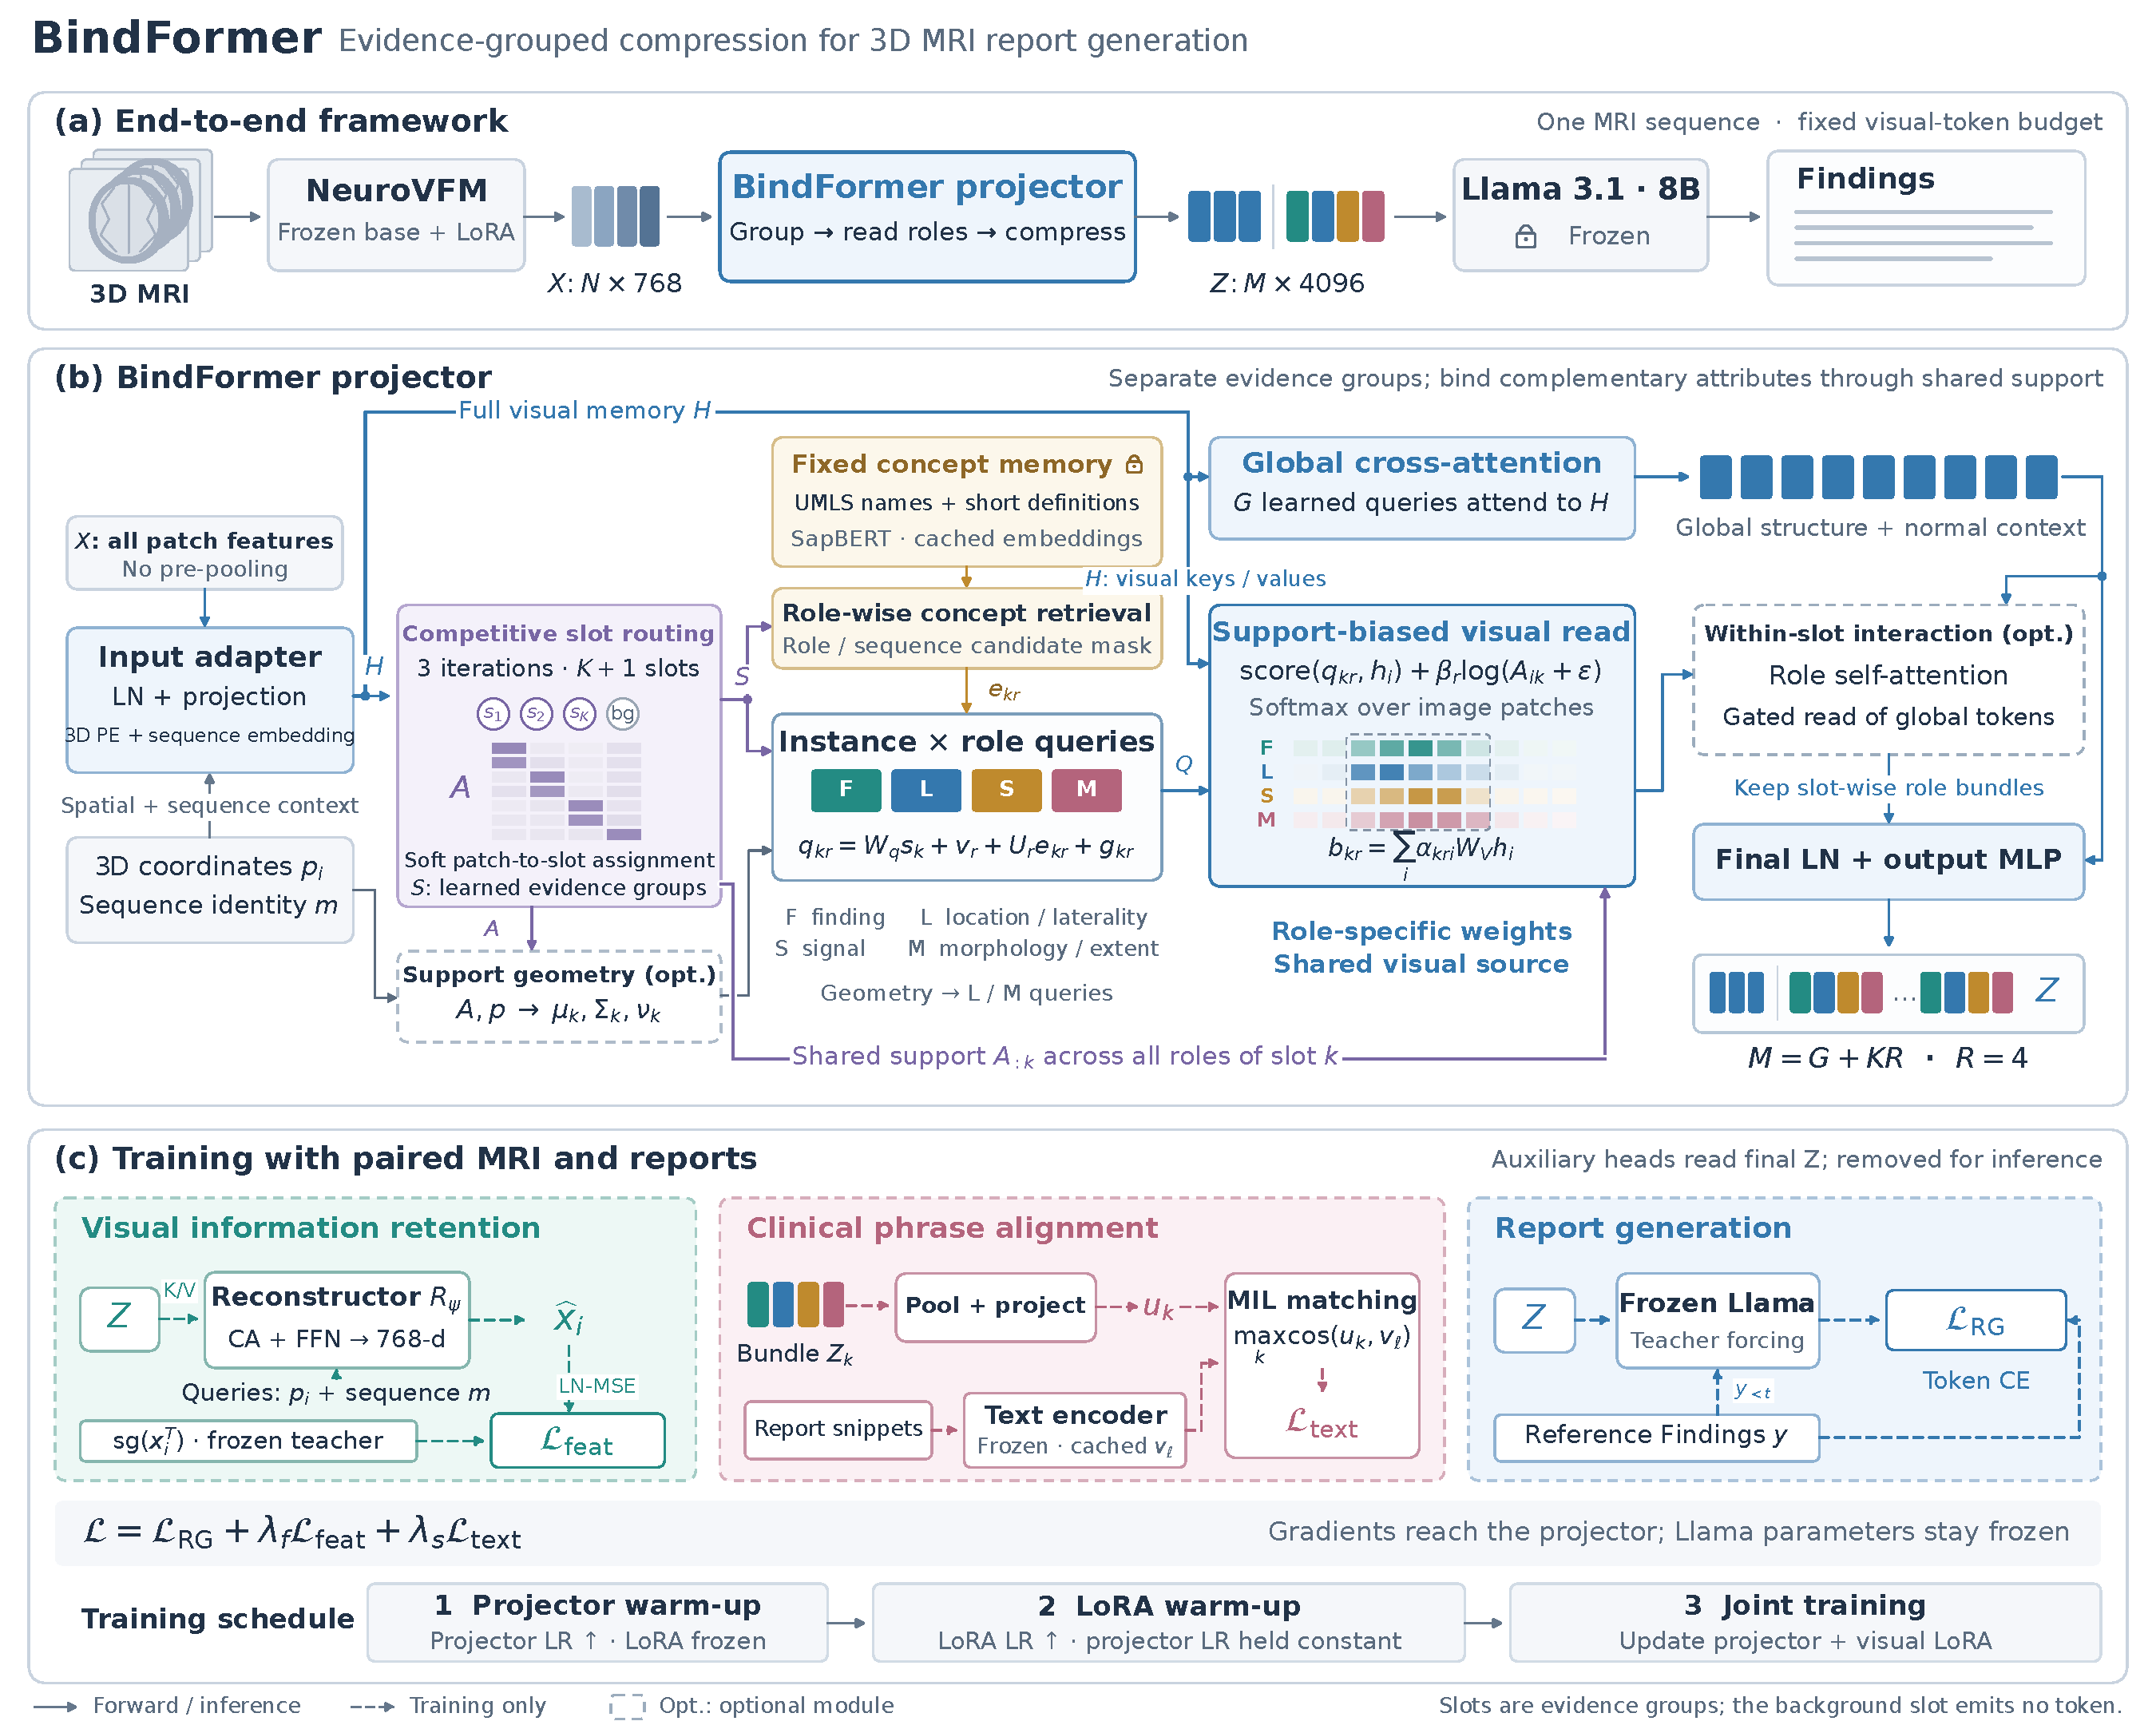
\includegraphics[width=\textwidth]{figures/bindformer_overview/bindformer_overview.pdf}
  \caption{\textbf{Overview of BindFormer.}
  (a) A single-sequence 3D MRI is encoded by NeuroVFM and compressed into a
  fixed number of continuous visual tokens for report generation with a
  frozen Llama decoder.
  (b) Competitive slot routing organizes the full patch memory into learned
  evidence groups and a background slot. Each non-background slot produces
  finding, location/laterality, signal, and morphology/extent queries.
  Role-specific retrieval from a fixed concept memory supplies semantic
  guidance; optional support geometry supplies spatial cues. A shared
  patch-to-slot assignment biases visual cross-attention so that different
  roles draw on a common evidence group while retaining distinct attention
  weights. The first role read uses image-derived values, with no direct
  residual from concept-conditioned queries. Global queries retain overall
  context. Optional within-slot self-attention and gated global-context
  reading refine local bundles before the output projection. With one query
  per role, the token budget is $M=G+KR$, where $R=4$; the background slot
  emits no output token.
  (c) Report generation loss $\mathcal{L}_{\mathrm{RG}}$ is combined with
  feature reconstruction $\mathcal{L}_{\mathrm{feat}}$ and report-fragment
  alignment $\mathcal{L}_{\mathrm{text}}$. Both auxiliary branches read the
  final projected tokens $Z$. The reconstruction head predicts features at
  sampled positions using $Z$, coordinates, and sequence identity, supervised
  by fixed features $X^T$ from the frozen NeuroVFM base. Text alignment matches
  complete role bundles to frozen report-fragment embeddings through a
  multiple-instance score. Negative-candidate construction is omitted from
  the illustration. Training comprises projector warm-up, visual-LoRA warm-up
  with the projector learning rate held constant, and subsequent joint
  training. Llama remains frozen, while gradients propagate through it to
  the visual pathway. Auxiliary heads are removed for inference.}
  \label{fig:bindformer-overview}
\end{figure*}
